\chapter{Base de donnée}
	\label{lab:bdd}

\section{Présentation}

Nous avons développé cette base de données pour répondre à notre problématique en utilisant des données simulées, car 

	\subsection{avantages des bases de données simulées}



	\section{Modèles}

15 modèles générés à partir d'images TDM réelle (center hospitalier Lyon-SUD). 

Utilisation du XCAT~\cite{segars2009mcatoverview}.

\todo{inclure image}
		\subsection{Respiration}


Pour prendre en compte la variabilité du cycle respiratoire (voir figure \ref{fig:variabCycle}), nous avons utilisé 4 cycles différents pour modéliser la respiration du patient. Un signal respiratoire complet a été acquis sur une durée de plusieurs minutes à l'aide d'un spiromètre (voir \ref{lab:spirometre}). Nous avons extraits 3 cycles semblables correspondants à la phase de de respiration normale, ainsi qu'un cycle ``anormal'' pour prendre en compte une respiration irrégulière.

\begin{figure}
 \centering
 \begin{tabular}{c c}
 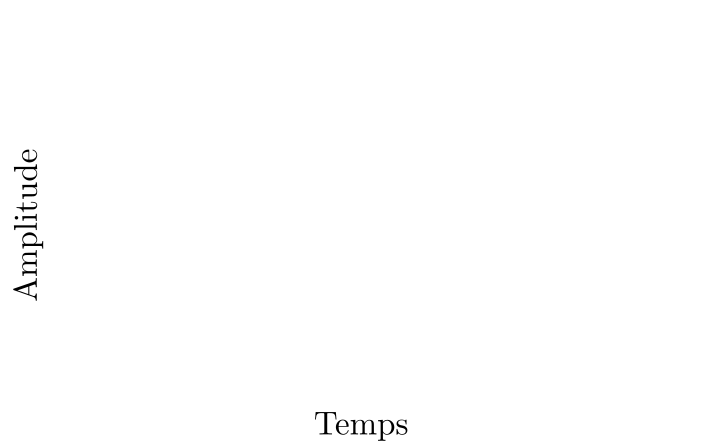
\includegraphics[width=8cm]{images/respiReguliere} &
 \includegraphics[width=8cm]{images/respiIrreguliere}
 \end{tabular}
 \caption[Exemple de courbes respiratoires régulière et irrégulière]{Deux exemples de courbes respiratoires prises par un spiromètre : La première montre une respiration régulière, tandis que celle du bas est irrégulière}
 \label{fig:variabCycle}
\end{figure}


La signal respiratoire obtenue est présentée dans la figure \ref{fig:cycleRespi}. Il est constitué de 4 cycles de 5.6 secondes qui se répètent 10 fois pour former un signal total de 224 secondes. 

Chacun de ces 4 cycle est discrétisé en 8 parties qui seront utilisées pour générer les modèles utilisés lors de la simulation. 


\begin{figure}
 \centering
 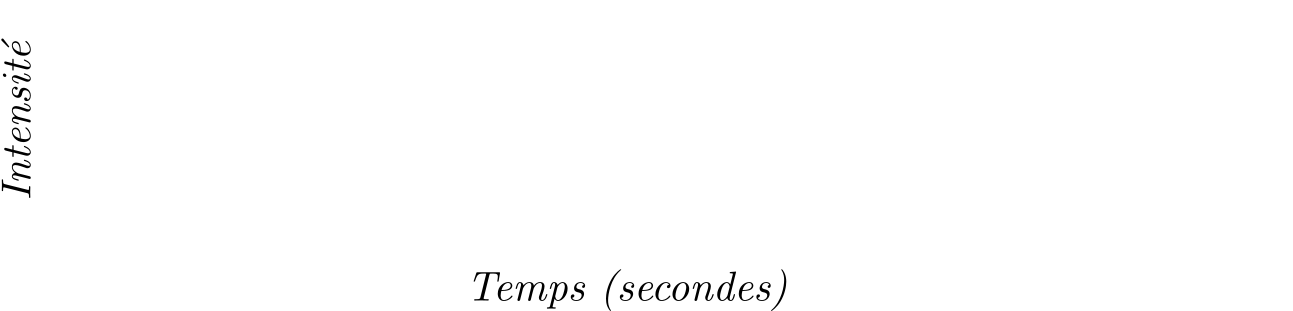
\includegraphics[width=8cm]{images/courbesRespi}

 \caption[signal respiratoire utilisé pour les modèles de la base de donnée]{Courbe respiratoire utilisée pour générer modèles respirant. Les traits verticaux du premier cycle montrent les 8 instants sélectionnés pour discrétiser le mouvement respiratoire de ce cycle.}
 \label{fig:cycleRespi}
\end{figure}

	\section{paramètres de simulation}

\subsection{Calibration de la base de données}

Notre but est de simuler des images avec un ensemble de tumeurs qui ne soient ni trop évidentes ni impossible à détecter. Nous avons donc cherché à obtenir une échelle de contrastes de tumeurs qui permettaient une détection par des humains de 10\%, 30\%, 50\%, 70\% et 90\%.

Pour réaliser cela, un ensemble d'images ont été simulées sans mouvement respiratoire, avec différentes tailles de tumeurs. Ensuite, une étude ROC avec deux observateurs humains non médecin est réalisée afin d'estimer la détectabilité de ces couples activité/taille de tumeurs (fig.\ref{fig:calibration}). 

Nous avons utilisé la base de donnée crée dans notre laboratoire et présentée dans~\cite{tomei2010oncopet_db}. Cette base de donnée contient entre autre 25 images TEP simulées à partir du modèle zubal~\cite{zubal1994computerized}, contenant 10 lésions par image. Ces lésions sont placées de manière aléatoire dans le poumon, les ganglions lymphatiques, le foie et la rate avec une probabilité de 30\% pour les 3 premiers organes et de 10\% pour la rate. Le contraste de ces lésions est déjà calibré pour une détection sur une échelle de 10\% à 90\%. Il y a donc 250 lésions, 75 dans les ganglions lymphatiques, 75 dans le foie, 75 dans le poumon, et 25 dans la rate. Nous n'avons réalisé notre étude que sur le foie et le poumon.

On présente à chaque observateur les images les unes après les autres, qu'ils vont annoter en recherchant toutes les lésions et en leur attribuant une note à l'aide du logiciel amide~\cite{loening2003amide}. Ils ne connaissent pas à l'avance la localisation des lésions, et doivent donner pour chaque lésion une note entre 1 et 5 correspondant au barème suivant :

\begin{enumerate}
\item Possible
\item Probable
\item Très probable
\item Pratiquement  certain
\item Certain
\end{enumerate}

\subsubsection{Étude de détectabilité}

Nous avons utilisé la base de donnée originale, avec les contrastes présentés en \ref{tab:contrastePoumonOrig} pour les lésions du poumon et \ref{tab:contrasteFoieOrig} pour les lésions du foie.

\begin{table}
\centering
\begin{tabular}{|c||c|c|c|c|c|}
 \hline
Poumon	& 10\% & 30\% & 50\% & 70\% & 90\% \\
\hline
4mm	& 2    &  5   &  8   & 10   & 13   \\
\hline
12mm    & 2    &  5   &  8   & 10   & 13   \\
\hline
16mm    & 2    &  3.5 &  4.5 & 7.5  & 10   \\
\hline
\end{tabular}

\caption[Contraste originaux des lésions du poumon pour létude de détectabilité]{Contrastes originaux appliqués aux lésions de la base OncoPET\_DB pour les tumeurs du poumon, avec les pourcentages de détection associés}
\label{tab:contrastePoumonOrig}
\end{table}

\begin{table}
\centering

\begin{tabular}{|c||c|c|c|c|c|}
 \hline
Poumon	& 10\% & 30\% & 50\% & 70\% & 90\% \\
\hline
4mm	& 2.5    &  4   &  4.5   & 6   & 9   \\
\hline
12mm    & 2    &  3   &  4   & 4.5   & 7.5   \\
\hline
16mm    & 2    &  3   &  4   & 4.5   & 7.5   \\
\hline
\end{tabular}

\caption[Contraste originaux des lésions du foie pour létude de détectabilité]{Contrastes originaux appliqués aux lésions de la base OncoPET\_DB pour les tumeurs du foie, avec les pourcentages de détection associés}
\label{tab:contrasteFoieOrig}
\end{table}

Lors de cette première étude, nous avons observé que les lésions de la base de donnée étaient beaucoup trop visibles, ce qui nous a amené à redéfinir les contrastes à utiliser pour la nouvelle version de la base de donnée. 

Deux observateurs non médecins ont marqué sur les 25 images de la base de donnée la localisation présumée de 10 lésions présentes dans le poumon, le sang, le foie et la rate.

Nous avons conservé les contrastes suivants pour deux diamètres de tumeurs :



\begin{table}

\centering

\begin{tabular}{|c||c|c||c|c|}
 \hline
	& 8mm Foie	& 12mm Foie	& 8mm Poumon	& 12mm Poumon	\\
\hline
10\%	& 1.8		& 1.3		& 3.0		& 2.5		\\
\hline
30\%	& 2.0		& 1.5		& 4.0		& 3.0		\\
\hline
50\%	& 2.5		& 1.8		& 5.0		& 3.5		\\
\hline
70\%	& 3.0		& 2.0		& 6.5		& 4.0		\\
\hline
90\%	& 3.5		& 2.3		& 8.0		& 5.0		\\
\hline
\end{tabular}
\caption[Contraste final lésions du foie]{Contrastes appliqués aux lésions en fonction du taux de détectabilité désiré}
\label{tab:contrasteFoieOrig}
\end{table}



\begin{figure}[h!]
\begin{center}
\includegraphics[width=15cm]{images/calibration}
\end{center}
\caption{Détectabilité des tumeurs réalisées par des humains en fonction du contraste et de la taille des tumeurs.} 
\label{fig:calibration}
\end{figure}

\todo{terminer etude de detectabilité : montrer les deux graphiques}

\subsubsection{Gestion des lits}

Le découpage des simulations en lits est nécessaire pour simuler de manière réaliste des acquisitions médicales. Or le logiciel de reconstruction avec correction de mouvement ne prenait pas du tout en compte la possibilité de découper les images en lits. 

J'avais supposé lorsque j'avais commencé à utiliser le logiciel que son créateur avait utilisé cette possibilité, mais il utilisait dans ses simulations une caméra virtuelle qui couvrait tout le patient. Cela a augmenté la complexité du système de reconstruction, car je devais réaliser autant d'estimation de mouvement qu'il y avait de lits.

\todo{gestion des lits .. peut-être plus dans la partie apport perso}

\section{Optimisation des paramètres de simulation}

L'optimisation des paramètres de reconstruction a été réalisée à partir d'une étude sur le rapport signal sur bruit des lésions.

Nous avons cherché le jeu de paramètres (Nombre d'itérations, Nombre de sous-ensemble) qui permettais de maximiser ce critère sur les images.

\section{Correction du mouvment}

\subsection{Images Statiques}

Les images statiques sont reconstruites à partir des donnés de simulation statiques, réalisées à partir d'une acquisition complète du modèle au premier instant du cycle respiratoire (fin d'expiration).

Elle est donc en phase avec la carte d'atténuation qui est elle aussi tirée du modèle en fin d'expiration.

\subsection{Images Non corrigées}

Les images non corrigées sont produites de la même manière que les images statiques, mais à partir des fichiers list-mode dynamiques.

\subsection{Estimation du mouvement respiratoire}

Pour estimer les mouvement respiratoire, nous avons décider d'utiliser les images TEP, car cette technique nous permet d'ajouter une imprécision réaliste. Les données dynamiques sont utilisées pour la reconstruction.

Les 8 images correspondant aux 8 instants du cycle moyen sont reconstruites séparément sans correction d'atténuation. Nous réalisons ensuite un recalage de chaque image sur l'image de référence (la première) à l'aide d'un algorithme de recalage élastique par B-splines. Le recalage est réalisé dans les deux sens, de manière à éviter de devoir inverser un des champs de mouvement.

Les champs de mouvement estimés vont permettre la correction du mouvement des images. 

Pour permettre une meilleur adéquation des données dynamiques avec la carte d'atténuation, elle est déformée à l'aide des champs de mouvement pour correspondre aux différents instants du cycle respiratoire.

\subsection{Images TE-MS}

Ces images sont reconstruites à l'aide d'un logiciel fourni par le LatIM~\cite{lamare2007list}, qui prend en compte l'estimation de mouvement réalisée précédemment ainsi que les fichiers list-mode générés par la simulation dynamique pour reconstruire directement les images corrigées. Les 8 cartes d'atténuation déformées sont fournies de manière à réaliser une reconstruction optimale.

\subsection{Images TI-IM}

Les 8 images correspondant aux 8 instants du cycle moyen sont reconstruites séparément à l'aide de la carte d'atténuation recalée correspondante. Puis toutes ces images sont déformées sur l'image correspondant au premier instant du cycle à l'aide de la carte de mouvement estimée précédemment.

Ces 8 carte recalées sont ensuite sommées pour obtenir les images corrigées.


	\section{données clef} % temps de calculs etc....

\subsection{Lésions}

\begin{table}
\centering
 \begin{tabular}{|c|c||c|c|c|c|c|} 
\hline
\multicolumn{2}{|c|}{Niveau de confiance}       & 1	  & 2	    & 3	     & 4	& 5	\\
\hline
\hline
Poumon	(173)	& 8 mm (90)	& 3 (19)  & 4 (18)  & 5 (18)  & 6.5 (18)	& 8 (17)\\
\cline{2-7}
		& 12 mm	(83)	& 2.5 (16)& 3 (16)  & 3.5 (18)& 4 (17)	& 5 (16)\\
\hline
Foie 	(107)	& 8 mm (54)		& 1.8 (11)& 2 (11)  & 2.5 (10)& 3 (11)	& 3.5 (11)\\
\cline{2-7}
		& 12 mm	(53)	& 1.3 (10)& 1.5 (10)& 1.8 (11)& 2 (11)  & 2.3 (11)\\
\hline 
 \end{tabular}

\caption[Tableau récapitulatif des lésions]{Tableau récapitulatif des contrastes des lésions présentes dans le foie et les poumon des modèles. Le nombre en parenthèse correspond au nombre de lésions}
\label{tab:contrastePoumonFoieRecap}


\end{table}

\subsection{activité des organes}


Les activités des organes sont décrites dans la table \ref{tab:contrastePoumonFoieRecap}
\begin{table}
\centering
 \begin{tabular}{|c|c|c|} 
\hline
Organe 		& Activité ($Bq/c^3$) & origine\\
\hline
\hline
Foie		& 7740		      & \\
\hline
Myocarde	& 11610		      & \\
\hline
Os		& 3863		      & \\
\hline
Poumon 		& 1338 		      & \\
\hline
Prostate	& 2575		      & \\
\hline
Rate		& 4939		      & \\
\hline
Reins		& 8220		      & \\
\hline
Sang		& 5340		      & \\
\hline
Tissus mous 	& 2575 		      & \\
\hline
Urètre		& 33815		      & \\
\hline
Vésicule bilaire& 2575		      & \\
\hline
Vessie		& 50973		      & \\
\hline
 \end{tabular}

\caption[Activités des organes des patients de la base de donnée]{Activités définies pour les organes des patients virtuels}
\label{tab:contrastePoumonFoieRecap}
\end{table}

15 modèles crées depuis 15 images TDM

Le temp de simulation nécessaire pour générer une image statique est de 130h pour un cpu environ, et 110 heures pour générer une image dynamique.

VOlume de données : bcp
